% !TeX spellcheck = en_GB

\section{Problem 4}

In what follows, we present the development process of our recipes search engine. We will focus on techniques and technologies we used to implement it, giving to the reader some brief explanations of key Information Retrieval (IR) concepts. You can find the source code in the material attached with this documentation.\\\\
\textbf{Disclaimer}: to run our code, be sure to be on a Linux machine (or any other that allows you to run Bash scripts) and have Python 2.7 installed. Note that some additional Python modules are required (see following sections).


\subsection{Recipes gathering}

Our initial approach was to implement a Python crawler to gather all the 11300 recipes that BBC site\cite{bbc} provides. We decided to use \textit{urllib2}\cite{urllib2} module to download .html pages containing recipes info and \textit{BeautifulSoup}\cite{beaut_soup} module to parse them and get links to other recipes.\\
Even though we succeeded in building a quite good crawler, we soon realized that this approach gave us no guarantees of downloading all recipes in the site and that it would take a lot of time to check which were the missing ones. Therefore, we looked for a better approach and found out that BBC exposes an .xml sitemap that gathers all the links to web pages of the site. At that point we were able to extract from that file all the relevant links, using \textit{BeautifulSoup}\cite{beaut_soup} utilities and regexes. You can find the code we used for this purpose in \textit{list\_recipes.py}.\\
The Python script we used was made to write recipes links to a .txt file. Then, we wrote a simple Bash script (\textit{download\_recipes.sh}) to process this file and download the recipes using \textit{wget} command. The real strength of this approach was that we were able to decide whether all recipes had been downloaded or not (due, for instance, to network issues) by checking downloaded files against the list of recipes urls (see \textit{check\_recipes.sh}).\\
To run our scripts, open a terminal and type
\begin{lstlisting}
	$ python list_recipes.py
	$ ./download_recipes.sh
\end{lstlisting}
Note that the entire download process could take more or less 4 hours to terminate. To check the result, type
\begin{lstlisting}
	$ ./check_recipes.sh
\end{lstlisting}
In case any recipe was not downloaded, the script will output the list of related urls and you can restart the download process (only for missing ones).


\subsection{Pre-processing}

In order to pre-process recipes, we first needed to extract from downloaded .html pages relevant informations.  Even in this case, we used \textit{BeautifulSoup}\cite{beaut_soup} utilities to parse them. Then, we stored obtained info in a big .tsv file, where each row represented a recipe, using \textit{unicodecsv}\cite{csv} module. You can find the code we used for this purpose in \textit{store\_recipes.py}. To run the script, open a terminal and type
\begin{lstlisting}
	$ python store_recipes.py
\end{lstlisting}
Note that the process could take more or less 15 minutes to terminate. Resulting file (\textit{recipes.tsv}) should appear like in the picture below.
\begin{center}
	\vspace{5mm}
	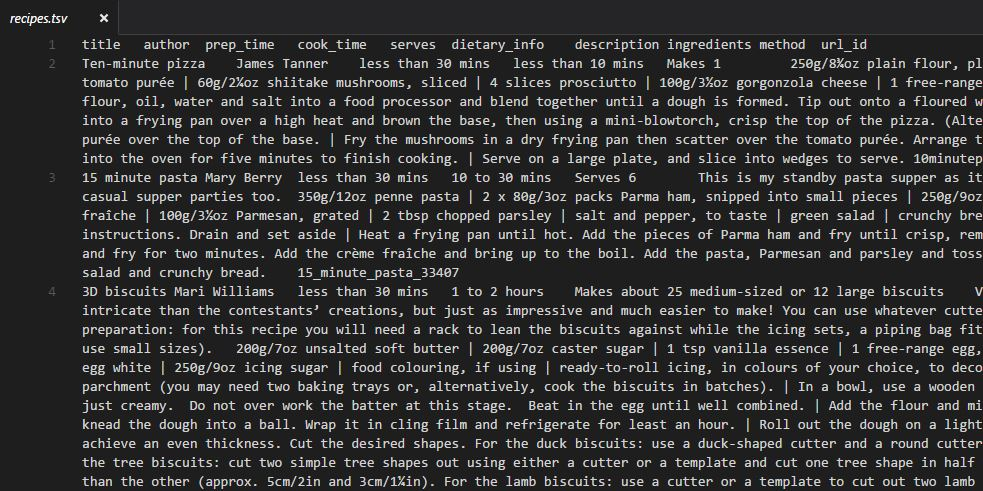
\includegraphics[scale=0.3]{img/recipes-tsv.jpg}
\end{center}
On that result, we applied pre-processing techniques using \textit{NLTK}\cite{nltk} library. We created a separated Python module (named \textit{preprocessing.py}) encapsulating all pre-processing logic, to be able to reuse it also in query processing part. In particular, this module includes functions implementing:
\begin{itemize}
	\item Tokenization
	\item Normalization
	\begin{itemize}
		\item remove diacritics.
		\item remove non-alphanumeric characters.
		\item convert text to lowercase.
		\item convert special unicode characters (e.g. fractions) into a somewhat "equivalent" ASCII representation.
	\end{itemize}
	\item Stopwords removal
	\item Stemming
\end{itemize}
Then, we made another script to store pre-processing result into another big .tsv file. You can find the code we used for this purpose in \textit{preprocess\_recipes.py}. To run the script, open a terminal and type
\begin{lstlisting}
	$ python preprocess_recipes.py
\end{lstlisting}
Resulting file (\textit{recipes-prep.tsv}) should appear like in the picture below.
\begin{center}
	\vspace{5mm}
	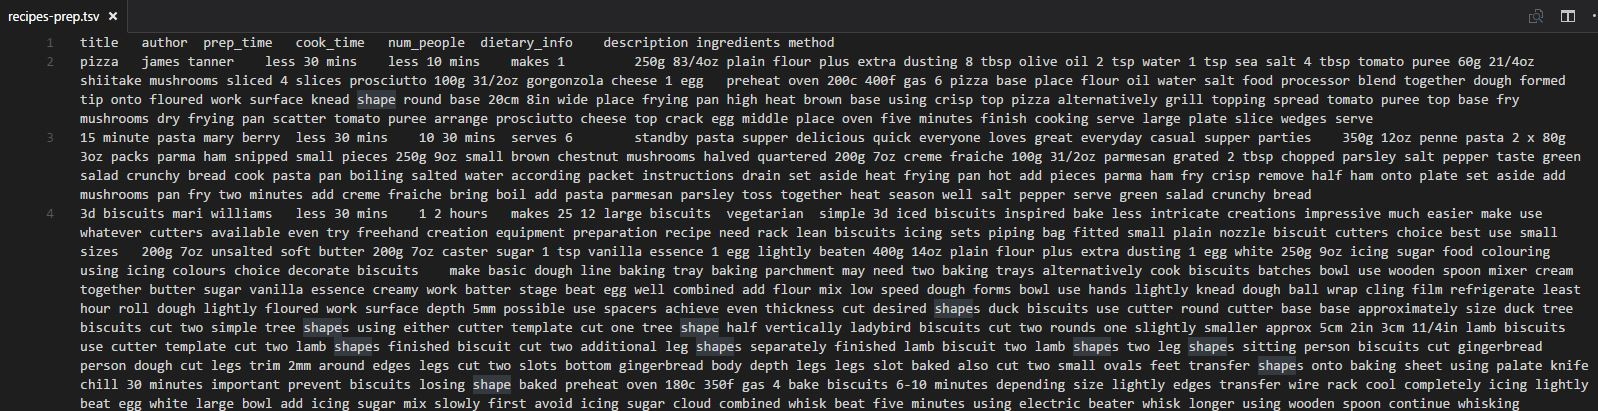
\includegraphics[scale=0.3]{img/recipes-prep-tsv.jpg}
\end{center}


\subsection{Inverted index building}

An Inverted Index\cite{inv_ind} is a particular data structure storing a mapping from words in a corpus of documents to their locations (i.e. in which documents they occur). We needed such that structure to perform proximity queries on our recipes corpus, using cosine-similarity measure. You can find the code we used for this purpose in \textit{build\_index.py}.\\
Basically, we developed a script that scans the whole corpus, building as you go both the doc-term (sparse) matrix\cite{doc_term} and its transpose, i.e. the index. The index is represented as a Python dictionary, in which an entry has following structure:
\begin{center}
	\textit{(term, list of postings pairs)}
\end{center}
A \textit{posting pair} is represented as a 2-items Python list \textit{(doc\_id, tf)}, where:
\begin{itemize}
	\item \textit{doc\_id} is the document id.
	\item \textit{tf} is the term frequency (i.e. number of times term occurs) in \textit{doc\_id}.
\end{itemize}
Note that the list is sorted with respect to \textit{doc\_id}.\\
The doc-term matrix is represented as a Python list of documents (i.e. the rows). Each row is a sparse vector, implemented with a Python dictionary in which an entry has following structure:
\begin{center}
	\textit{(term, tf)}
\end{center}
For the sake of memory efficiency, we made the two data structures share their entries. Indeed, matrix cells (instead of the single tf value) actually contain (a reference to) the corresponding posting in the index. Therefore, the script scans the documents in the corpus, updating as you go the value of \textit{tf} of the terms it encounters.\\
Note that we needed doc-term matrix to perform an optimization of the index for query processing: for each posting in a term posting list, we want to store the complete query-independent factor, i.e.
\begin{align*}
	tf_{term,doc} * \dfrac{idf_{term}^2}{||doc||}
\end{align*}
where $idf_{term}$ is the Inverse Document Frequency\cite{tf_idf} of the term, and $||doc||$ is the length of the vector representing the document.\\
To run the script, open a terminal and type
\begin{lstlisting}
	$ python build_index.py
\end{lstlisting}
The result a dump of both the doc-term matrix and the index to separated .pickle files (we used \textit{pickle}\cite{pickle} module to do that). This allows to easily recreate the index in memory when needed for query processing. 


\subsection{Query processing}

To make queries against our corpus of recipes we built a Python module (named \textit{query\_processing.py}) encapsulating all the logic and algorithms needed to process them. Then, we created a simple command line interface (\textit{process\_queries.py} module) through which we are able to submit a query and get the related recipes, presented in a structured way.\\
Our initial approach consisted in providing only disjunctive queries. Indeed, for instance, a query like \textit{"butter apple banana"} returned the (at most) 20 most related recipes (according to cosine-similarity) that contained \textit{at least one} of the words in the query. It was trivially achieved by selecting the posting lists related to each of the terms, computing their union, computing the score for each document (using the related query-independent factor stored in the index) in it and getting the ids of the (at most) 20 documents with the highest scores. Note that queries are first preprocessed using the same techniques we used for recipes. Documents contents retrieval is performed by scanning \textit{recipes.tsv} files, collecting as you go the rows of interest (using resulting documents ids).\\
At that point, we were satisfied about the performances of the system, since in average a query was answered in the order of the tenth of second. Therefore, we decided not to perform further optimizations and proceed implementing some extra features.


\subsubsection{Advanced features}

We decided to extend the set of provided query types, by also allowing terms conjunctions and negation. In order to do that, we introduced some operators, denoted by sequences of special characters, and a precise syntax rule to use them. In the end, the following was the prototype of query admitted by our system
\begin{align*}
	\text{t1 t2 t3 }\ldots \ [ \ || \text{ t4 t5 } \ldots \ || \ \ldots \ || \text{ t6 }\ldots \ ] \ [ \text{ *vegetarian } | \text{ *vegan }] \ [ \text{ -t7 -t8 }\ldots \ ]
\end{align*}
Terms separated only by a blank space are assumed to be in conjunction. Note that blocks surrounded by square brackets are optional. The operators we introduced are:
\begin{itemize}
	\item $||$ , disjunction operator. Sequences of terms separated by this operator are assumed to be in disjunction.
	
	\item $-$ , negation operator. Terms preceded by this operator should not appear in resulting documents.
	
	\item $*$ , keyword operator. Terms preceded by this operator represents keywords of our systems. The result of a keyword evaluation is its substitution with a sequence of predefined negated terms. It is a shortcut to exclude from resulting documents those which are not compliant with the given dietary habits.
\end{itemize}
In order to accept this type of queries, we added before preprocessing a preliminary phase of query parsing. In this way, we could extract the negated terms and the conjunctive groups, and process them individually, merging the results at the end. To process a conjunctive group, we iteratively applied the "merging intersect algorithm" described in \cite{iir} (ch. 1, pag. 11). Then, to compute the disjunction of all groups, we applied "merging union algorithm" described in \cite{iir} (). In the end, we discarded the documents that contained negated terms.\\
In addition, we gave different weights depending on in which "field" of the recipe it occurs. For instance, a term appearing in the title is much more relevant than the same term occurring in the method.




















\subsubsection{Instructions to run}

To run the command line interface, open a terminal and type
\begin{lstlisting}
	$ python process_queries.py
\end{lstlisting}
Note that the system takes some seconds at the beginning to load the index in memory from storage. Then, follow instructions to write a legal query. You can exit the program by simply pressing Enter without inserting text (or forcing process termination as well).
